\documentclass{beamer}
\setbeamertemplate{navigation symbols}{}

% there's no great way to make these "print-able"
\usetheme{Madrid}
\usecolortheme{beaver}
%\geometry{letterpaper,landscape}

% packages
\usepackage{graphicx}
\usepackage{hyperref}

% metadata
\title{Portfolio}
\author{Vaughn Kottler}
\date{\today}

% Link reference styling: blue, underlined with underline close to text
\newcommand{\HREF}[2]{{\color{blue}\underline{\smash{\href{#1}{#2}}}}}

\begin{document}

%%%%%%%%%%%%%%%%%%%%%%%%%%%%%%%%%%%%%%%%%%%%%%%%%%%%%%%%%%%%%%%%%%%%%%%%%%%%%%%
%                                 About Me                                    %
%%%%%%%%%%%%%%%%%%%%%%%%%%%%%%%%%%%%%%%%%%%%%%%%%%%%%%%%%%%%%%%%%%%%%%%%%%%%%%%

\begin{frame}
\frametitle{About Me}
    I am a senior Computer Engineering undergraduate student
    at the University of Wisconsin-Madison.
    \break

    My current passion is working on embedded electronics and software for
    vehicle systems. Designing such systems from scratch has revealed
    to me some of the technical and operational complexities in building a
    physical product.
\end{frame}

\begin{frame}
\frametitle{About Me}
    Iteratively deriving more efficient workflows and processes is a skill
    I have invested time developing and has helped me participate in a
    multitude of projects and work effectively with different technology
    stacks.
    \break

    I have a strong appreciation for ``test driven'' development and generally
    thinking through problems as thoroughly as possible before getting deep into
    the work because it tends to
    result in the most uninterrupted time spent doing the enjoyable, ``engineering'' parts.
\end{frame}

\begin{frame}
\frametitle{About Me}
    My home electronics lab when it was first set up
\begin{center}
    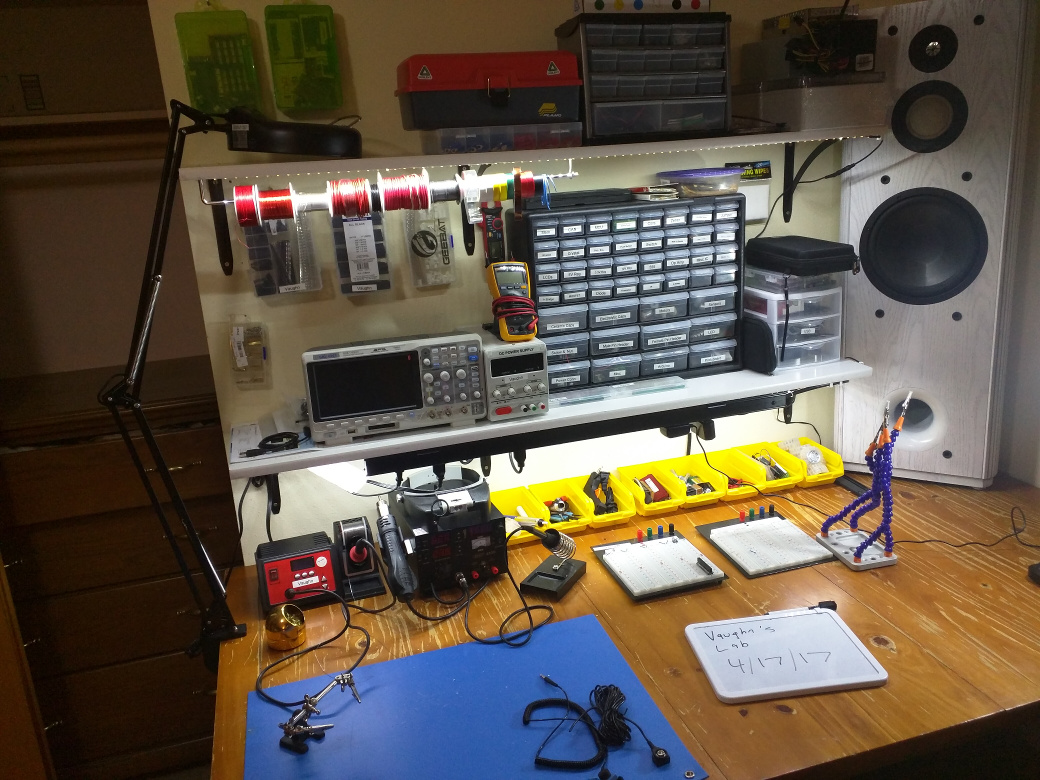
\includegraphics[width=3.5in]{assets/HomeLab}
\end{center}
\end{frame}

%%%%%%%%%%%%%%%%%%%%%%%%%%%%%%%%%%%%%%%%%%%%%%%%%%%%%%%%%%%%%%%%%%%%%%%%%%%%%%%


%%%%%%%%%%%%%%%%%%%%%%%%%%%%%%%%%%%%%%%%%%%%%%%%%%%%%%%%%%%%%%%%%%%%%%%%%%%%%%%
%                        Hyperloop II: Electrical System                      %
%%%%%%%%%%%%%%%%%%%%%%%%%%%%%%%%%%%%%%%%%%%%%%%%%%%%%%%%%%%%%%%%%%%%%%%%%%%%%%%

\begin{frame}
\frametitle{Hyperloop II: Electrical System}
\begin{center}
    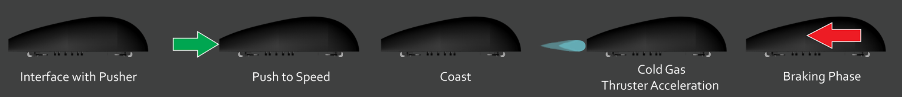
\includegraphics[width=\linewidth]{assets/badgerloop_2/conops}
\end{center}
    The image above captures the concept of operation of the second Badgerloop
    pod. It's a vehicle that must travel about one mile across a rail inside
    a vacuum.
    \break

    this particular vehicle used two COPVs filled to ~3000 PSI feeding a single
    ``converging-diverging'' nozzle.
    \break

    I was responsible for the embedded electronics and web-based user interface
    that would be used to view pod telemetry while it's inside the tube and
    send manual commands if/when necessary.
\end{frame}

\begin{frame}
\frametitle{Hyperloop II: Electrical System}
    Testing charging via the control panel
\begin{center}
    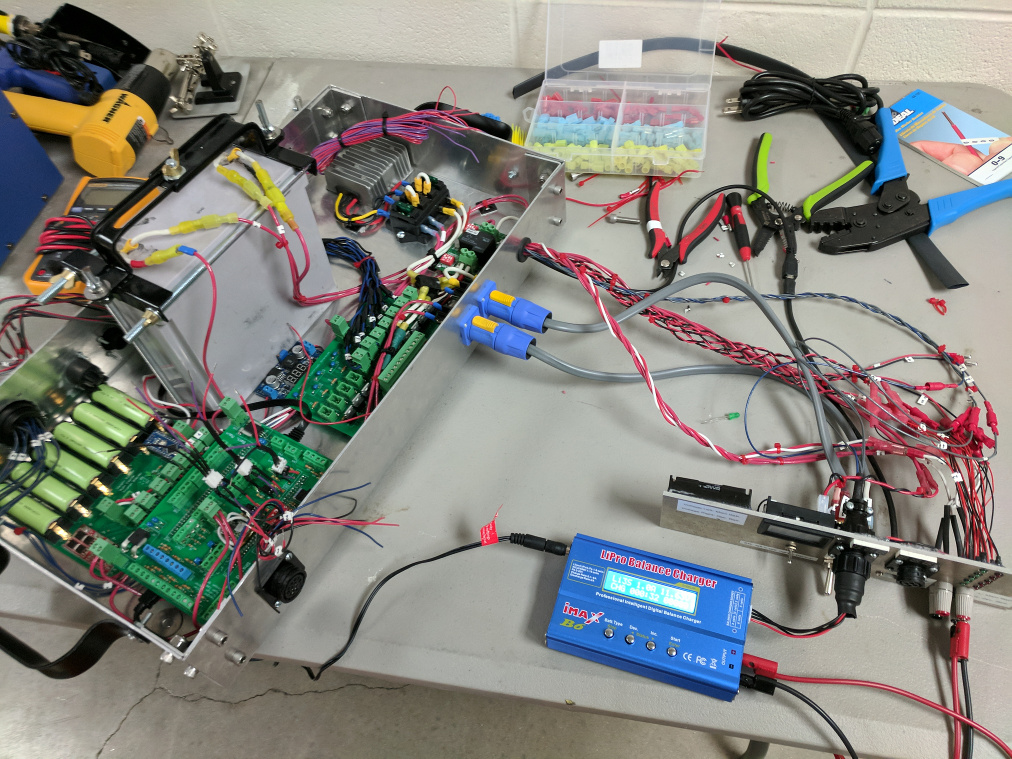
\includegraphics[width=3.5in]{assets/electrical_system/charging_test}
\end{center}
\end{frame}

\begin{frame}
\frametitle{Hyperloop II: Electrical System}
    Control panel for easy access to charging, programming and status LEDs
\begin{center}
    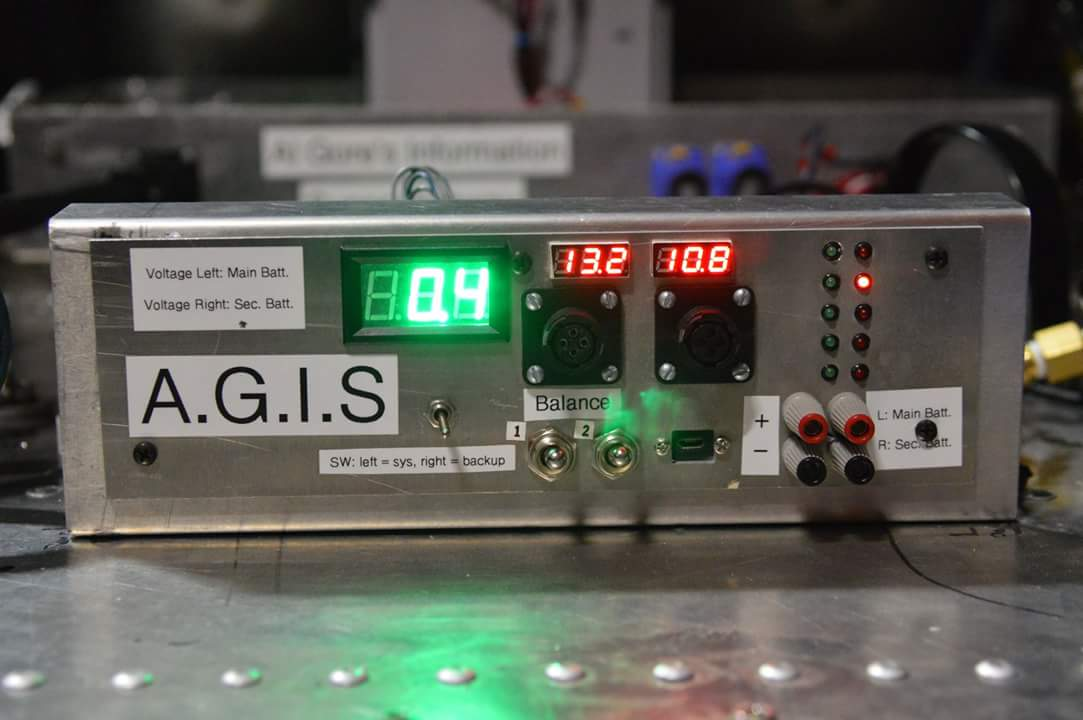
\includegraphics[width=3.5in]{assets/electrical_system/panel}
\end{center}
\end{frame}

\begin{frame}
\frametitle{Hyperloop II: Electrical System}
    Pod's entire electrical system in one image
\begin{center}
    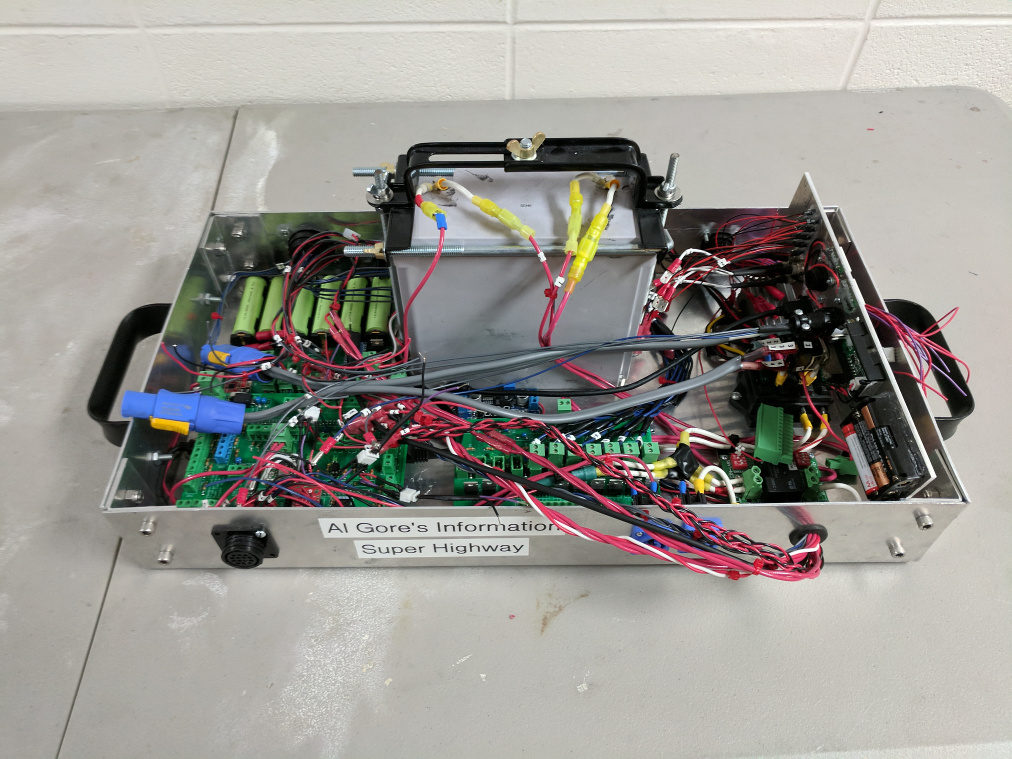
\includegraphics[width=3.5in]{assets/electrical_system/portability1}
\end{center}
\end{frame}

\begin{frame}
\frametitle{Hyperloop II: Electrical System}
    Battery and some harnessing removed for transport
\begin{center}
    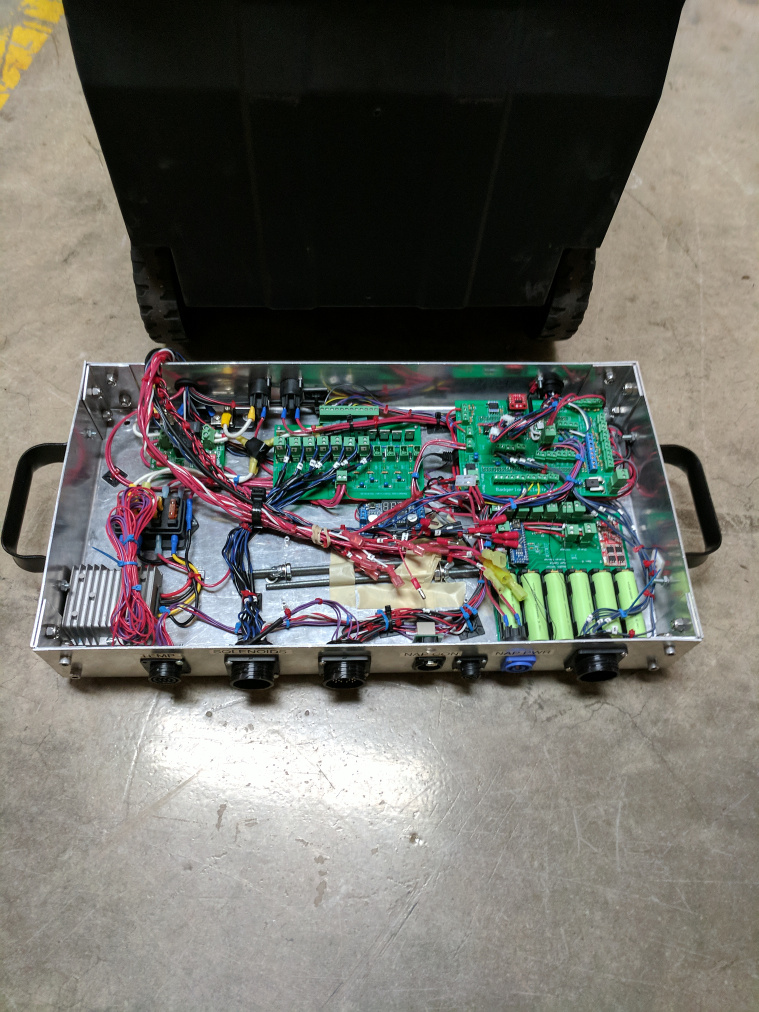
\includegraphics[width=2in]{assets/electrical_system/portability2}
\end{center}
\end{frame}

%%%%%%%%%%%%%%%%%%%%%%%%%%%%%%%%%%%%%%%%%%%%%%%%%%%%%%%%%%%%%%%%%%%%%%%%%%%%%%%


%%%%%%%%%%%%%%%%%%%%%%%%%%%%%%%%%%%%%%%%%%%%%%%%%%%%%%%%%%%%%%%%%%%%%%%%%%%%%%%
%                           Hyperloop II: Dashboard                           %
%%%%%%%%%%%%%%%%%%%%%%%%%%%%%%%%%%%%%%%%%%%%%%%%%%%%%%%%%%%%%%%%%%%%%%%%%%%%%%%

\begin{frame}
\frametitle{Hyperloop II: Dashboard}
The following slides include screenshots of the web-based dashboard I created
to monitor and control our pod for the second hyperloop competition (Summer 2017).
\break

The embedded system is one
\HREF{https://www.digikey.com/products/en/development-boards-kits-programmers/evaluation-boards-embedded-mcu-dsp/786}{STM32 Nucleo 144 F767ZI} 
microcontroller development board. We wrote all of the firmware
\HREF{https://github.com/madison-embedded/gcc-builds}{from-scratch}
and used \HREF{https://savannah.nongnu.org/projects/lwip/}{LwIP} to implement the network stack.
\break

The ``terminal'' shown in the following slides is ``redirected \texttt{stdout}'' from
the microcontroller, not an SSH session or userspace Linux program.
\break

Bootstrapping the microcontroller's serial terminal to a web-based UI is
the key feature of this UI.
\break

The dashboard source repository
\HREF{https://github.com/badgerloop-software/dashboard}{is here}.

\end{frame}

\begin{frame}
\frametitle{Hyperloop II: Dashboard}
    Console left (showing boot post and \texttt{help} command), data table right
\begin{center}
    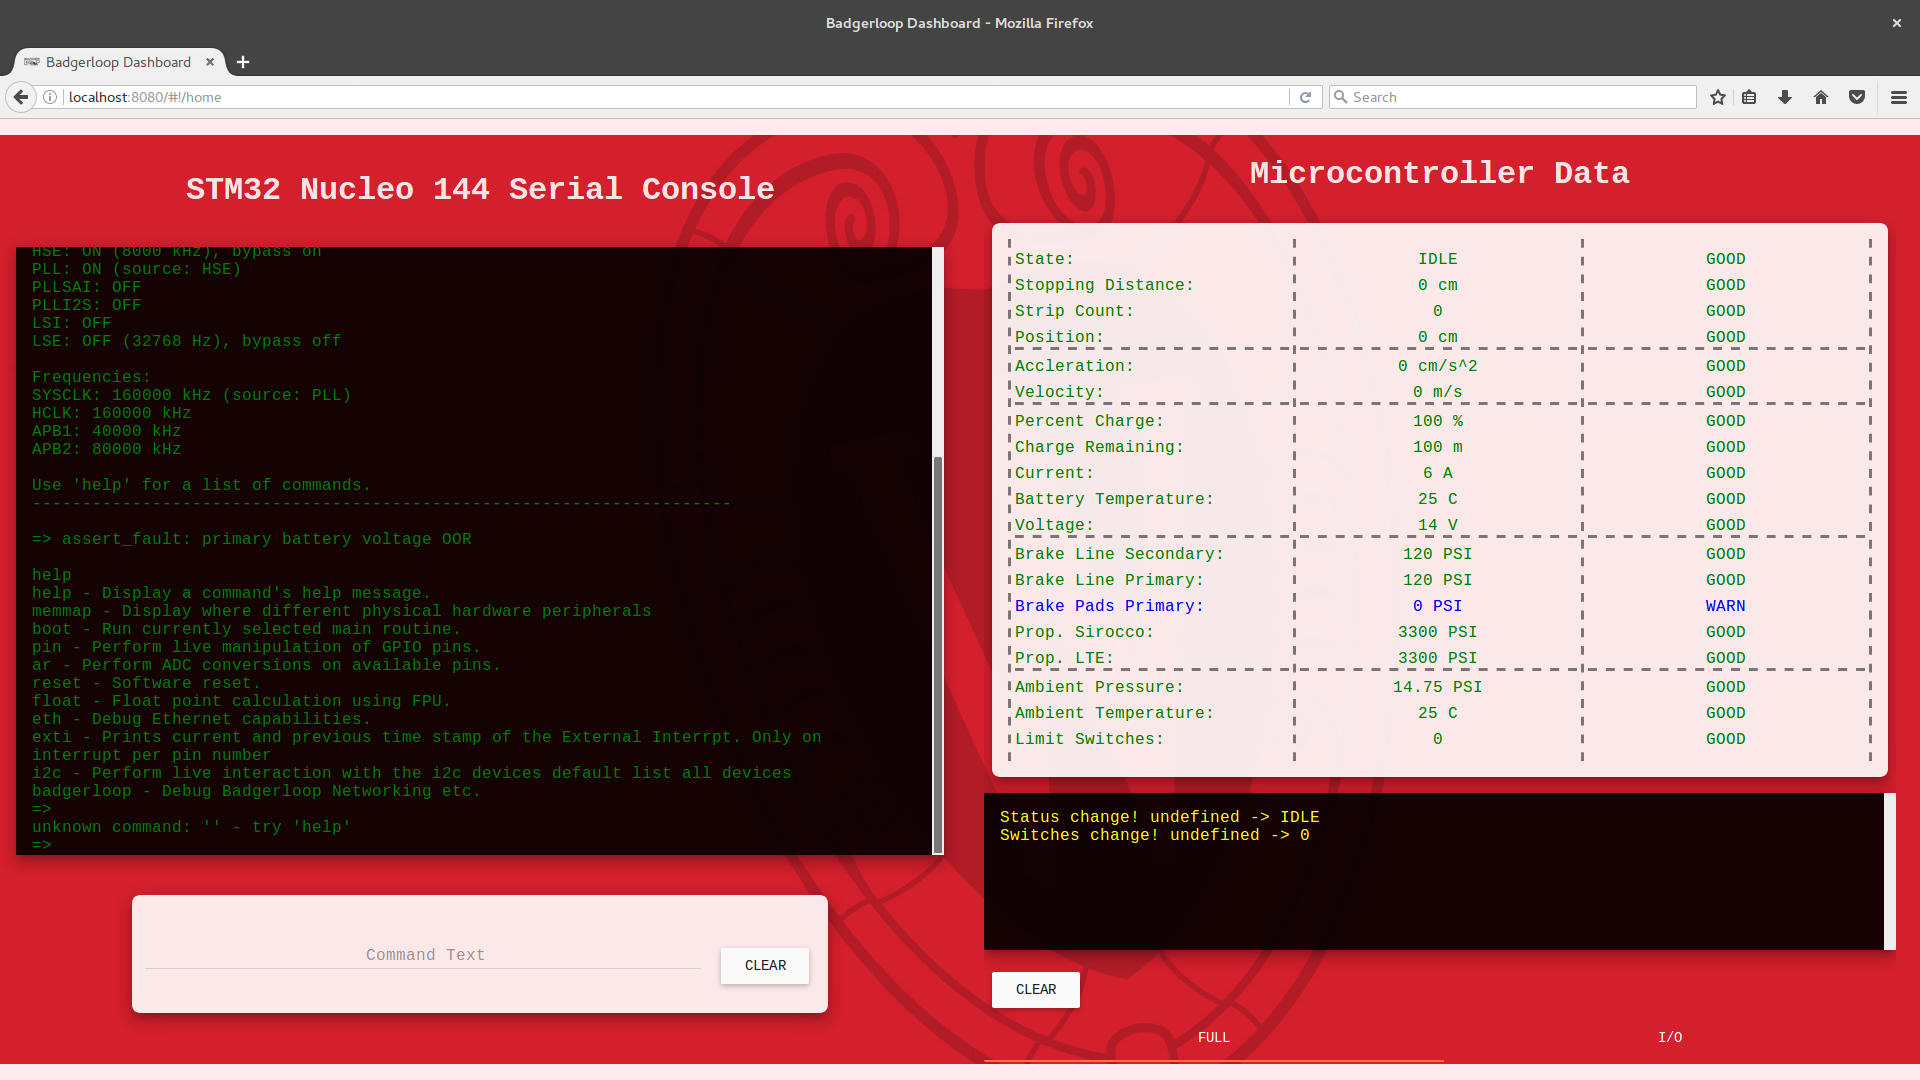
\includegraphics[width=\linewidth]{assets/badgerloop_2/Dashboard/dash_live1}
\end{center}
\end{frame}

\begin{frame}
\frametitle{Hyperloop II: Dashboard}
    Console left (showing post and \texttt{help} command), manual IO menu right
\begin{center}
    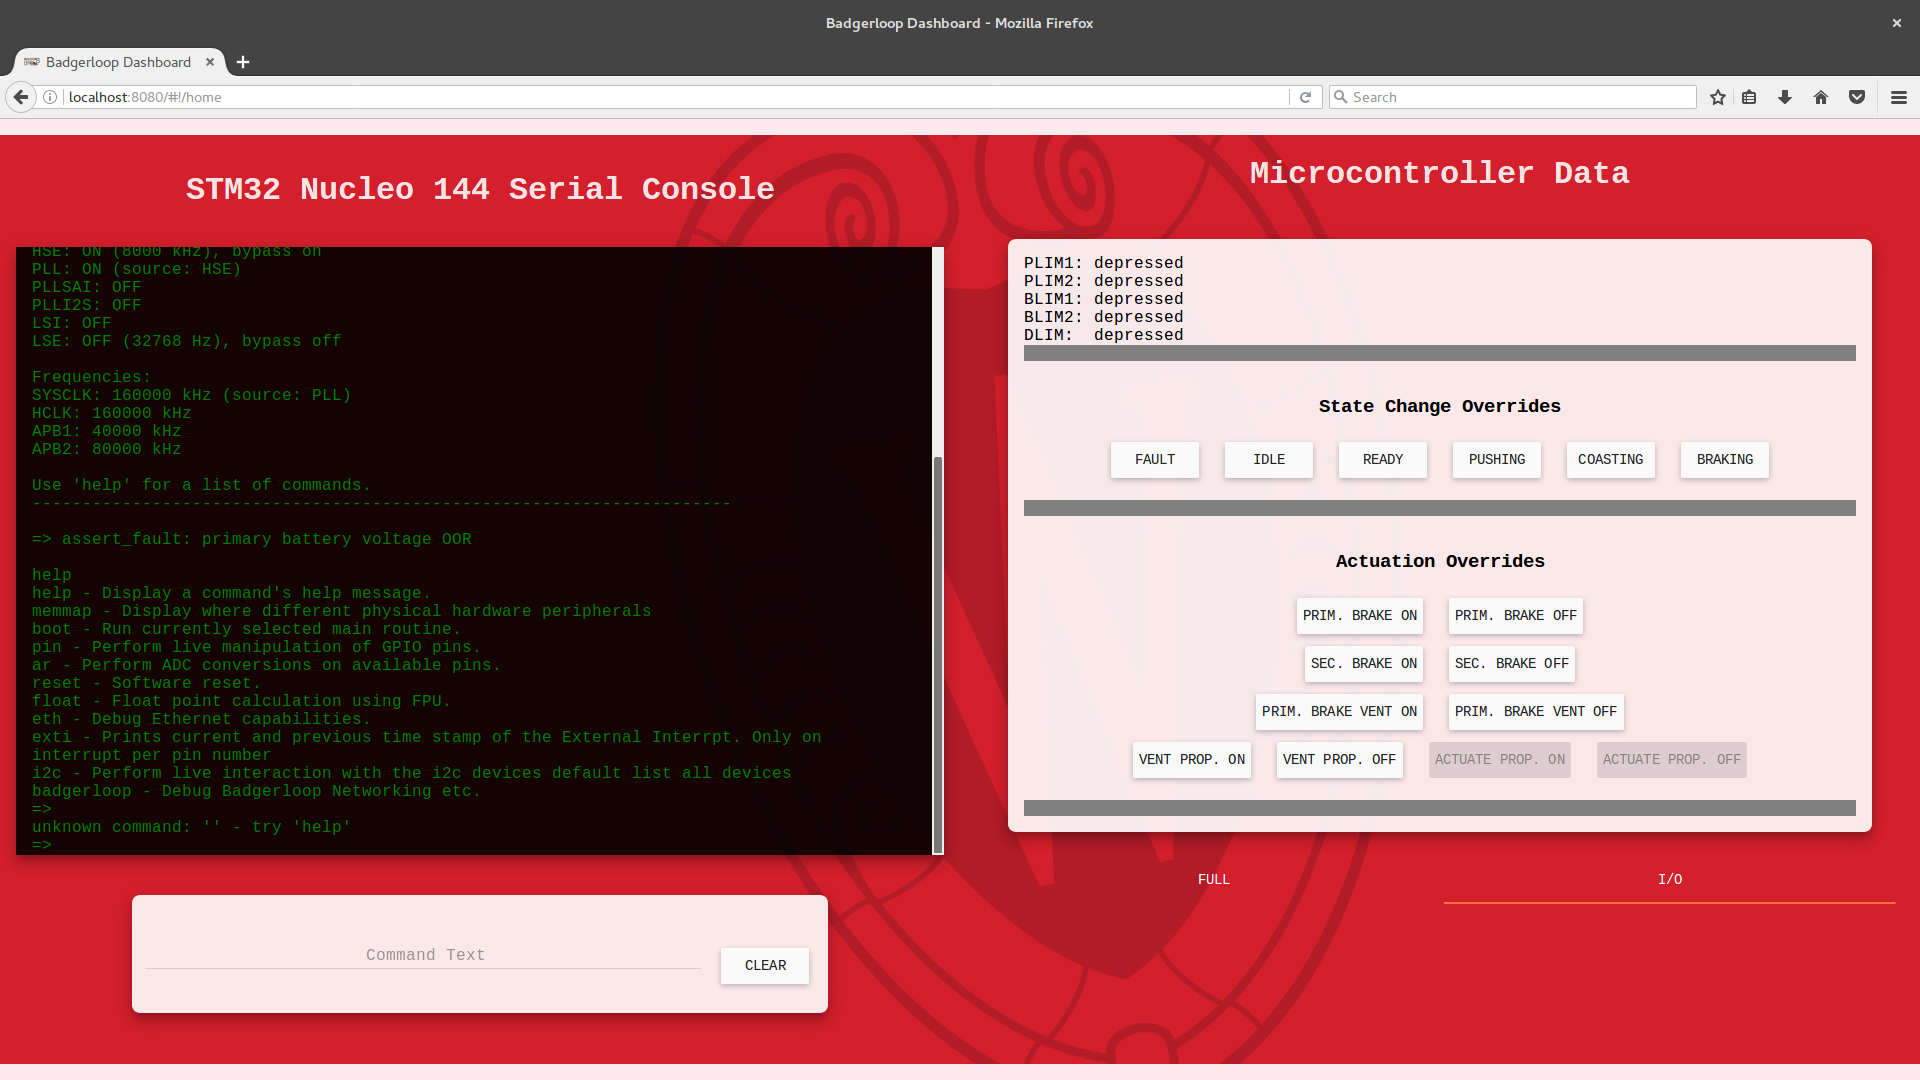
\includegraphics[width=\linewidth]{assets/badgerloop_2/Dashboard/dash_live2}
\end{center}
\end{frame}

\begin{frame}
\frametitle{Hyperloop II: Dashboard}
    \texttt{memmap} output and \texttt{badgerloop} sub-commands
\begin{center}
    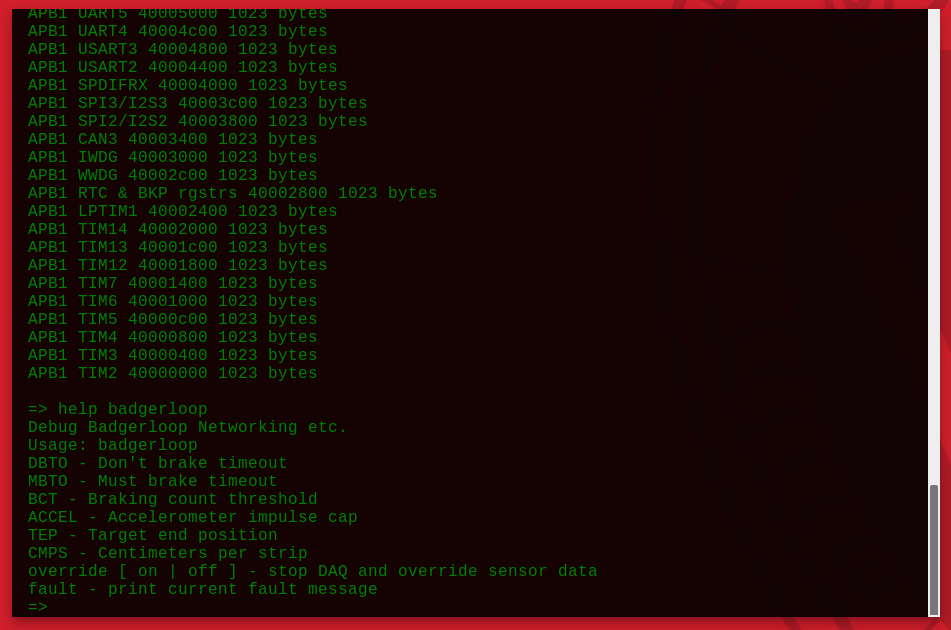
\includegraphics[width=4in]{assets/badgerloop_2/Dashboard/dash_cli_example}
\end{center}
\end{frame}

\begin{frame}
\frametitle{Hyperloop II: Dashboard}
    \texttt{ar} (analog read) command output, raw 10-bit ADC
\begin{center}
    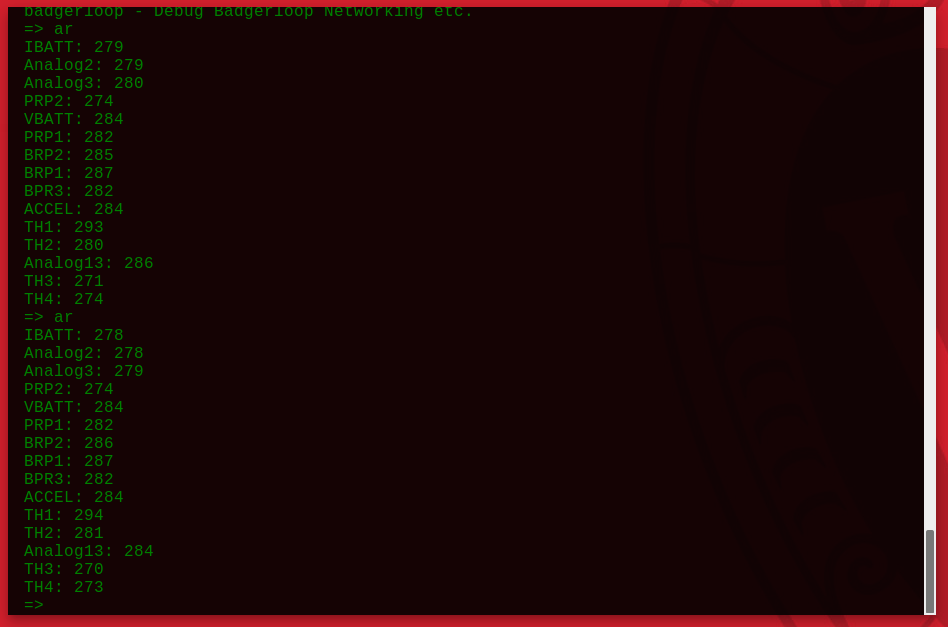
\includegraphics[width=4in]{assets/badgerloop_2/Dashboard/dash_live_ar}
\end{center}
\end{frame}

\begin{frame}
\frametitle{Hyperloop II: Dashboard}
    Development on the Dashboard on the road to the competition from Wisconsin
\begin{center}
    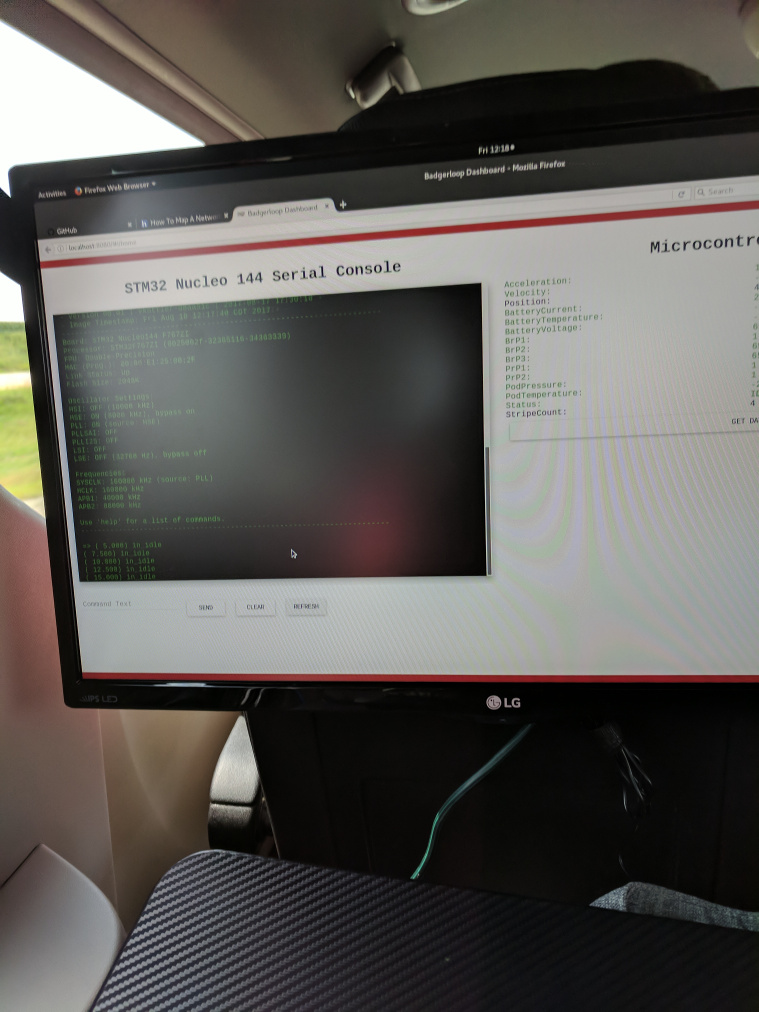
\includegraphics[height=2.5in]{assets/badgerloop_2/Dashboard/in_the_car}
\end{center}
\end{frame}

%%%%%%%%%%%%%%%%%%%%%%%%%%%%%%%%%%%%%%%%%%%%%%%%%%%%%%%%%%%%%%%%%%%%%%%%%%%%%%%


%%%%%%%%%%%%%%%%%%%%%%%%%%%%%%%%%%%%%%%%%%%%%%%%%%%%%%%%%%%%%%%%%%%%%%%%%%%%%%%
%                              Senior Design                                  %
%%%%%%%%%%%%%%%%%%%%%%%%%%%%%%%%%%%%%%%%%%%%%%%%%%%%%%%%%%%%%%%%%%%%%%%%%%%%%%%

\begin{frame}
\frametitle{Senior Design: Overview}
    Planning to update this with progress, right now the
    \HREF{https://github.com/vkottler/senior-design/blob/master/docs/proposal/proposal-final.pdf}{finalized proposal}
    and \HREF{https://github.com/vkottler/senior-design/blob/master/docs/proposal/presentation.pdf}{presentation slides}
    are complete and we're working on keeping
    additional \HREF{https://fault-tolerant-quadcopter.readthedocs.io/en/latest/}{online documentation} relevant.
    \break

    The goal is to build a quadcopter that communicates with a ground station
    and can be controlled and monitored through a web-based user interface.
    \break

    Design details are (currently) best captured by the proposal.
\end{frame}

\begin{frame}
\frametitle{Senior Design: Concept of Operation}
\begin{center}
    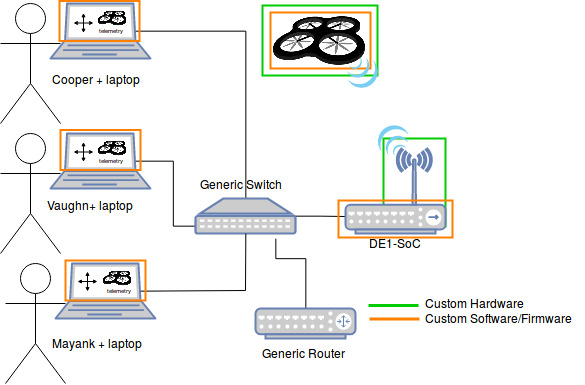
\includegraphics[width=3.5in]{assets/senior_design/conops}
\end{center}
    The essence of what we're working on
\end{frame}

\begin{frame}
\frametitle{Senior Design: Block Diagram}
    Quadcopter physical architecture
\begin{center}
    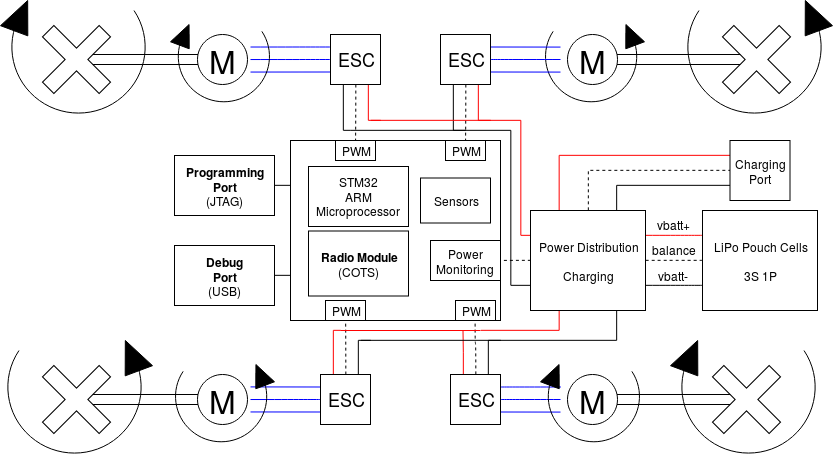
\includegraphics[width=\linewidth]{assets/senior_design/quadcopter}
\end{center}
\end{frame}

\begin{frame}
\frametitle{Senior Design: Block Diagram}
    Ground station software architecture and components
\begin{center}
    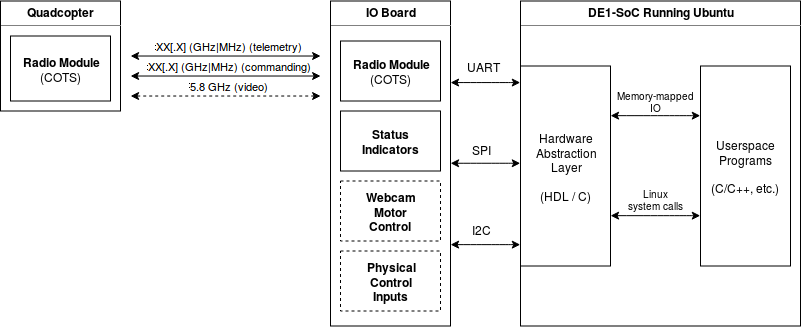
\includegraphics[width=\linewidth]{assets/senior_design/ground_station}
\end{center}
\end{frame}

\begin{frame}
\frametitle{Senior Design: Block Diagram}
    User interface software architecture
\begin{center}
    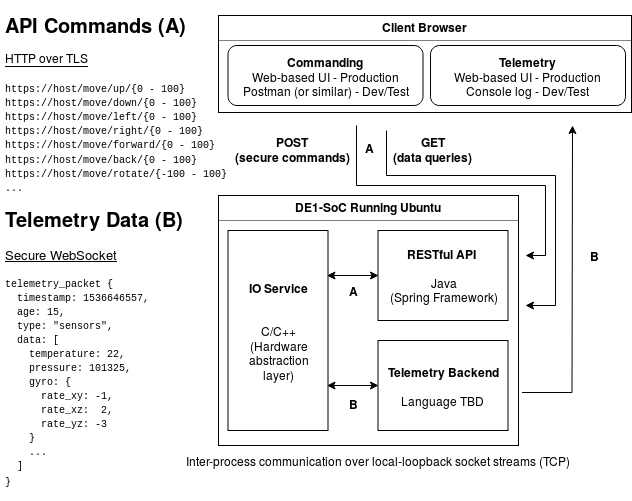
\includegraphics[width=3.5in]{assets/senior_design/display_controller}
\end{center}
\end{frame}

\begin{frame}
\frametitle{Senior Design: Power Supply Module}
    12V 2A input creates 5V and 3.3V rails with ``power good'' LEDs, just
    implements the reference design for a switch-mode and linear regulator
\begin{center}
    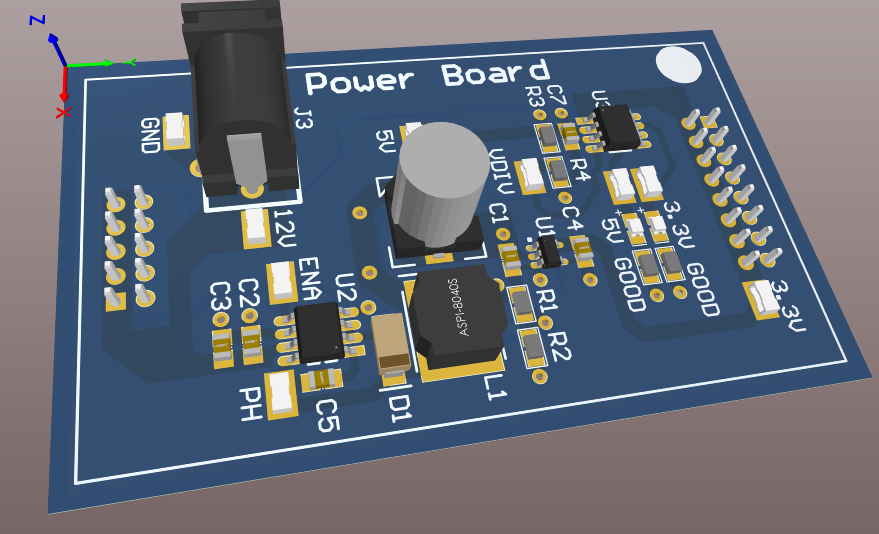
\includegraphics[width=3.5in]{assets/senior_design/power_3d}
\end{center}
\end{frame}

%%%%%%%%%%%%%%%%%%%%%%%%%%%%%%%%%%%%%%%%%%%%%%%%%%%%%%%%%%%%%%%%%%%%%%%%%%%%%%%

\end{document}
